\section{単精度実行} \label{sec:single}
%------------------------------------------------------








\section{地図投影法と計算領域の位置} \label{sec:adv_mapproj}
%------------------------------------------------------
計算領域の位置と投影法は、configファイルの\verb|PARAM_MAPPROJ|の項目を編集することで設定できる。
\textcolor{red}{\bf この設定も、pp\_***.conf、init\_***.conf、run\_***.confのconfigファイルの間で
必ず一致させなければならない。}はじめに下記の例をもとに説明する。\\

\noindent {\small {\gt
\ovalbox{
\begin{tabularx}{140mm}{l}
\verb|&PARAM_MAPPROJ| \\
\verb| MPRJ_basepoint_lon = 138.727778D0,| \\
\verb| MPRJ_basepoint_lat = 35.360556D0,| \\
\verb| MPRJ_type          = 'MER',| \\
\verb|/| \\
\end{tabularx}
}}}\\

\noindent まず\verb|MPRJ_basepoint_lat|と\verb|MPRJ_basepoint_lon|は、計算領域の中心の緯度・経度を表す。
SCALEでは、北緯を正、南緯を負の値として表現し、経度は0度を起点に右回りで表現するため、この設定では計算領域の
中心が北緯35.360556度、東経138.727778度に位置することになる。この場所を中心に指定された大きさで、計算領域が
設定される\footnote{デフォルトではメルカトル図法に基づいて緯度・経度を計算する際の基準とする緯度は、
MPRJ\_basepoint\_latの値が使用されるが、MPRJ\_M\_latを用いて任意の緯度を指定することもできる。}。
実際にはSCALE内部での格子点は実距離に基づいて格子点が配置されるので、投影法で設定されるのは、
実距離に基づいた緯度・経度座標が計算される。この緯度・経度情報は、すべてのSCALEのNetCDF形式の出力ファイルに
含まれている。

\verb|MPRJ_type|は、地図投影法の種類を表しており、\verb|MER|はメルカトル図法を意味する。
SCALEで現在選択できる地図投影法とその指定文字列は次のとおりである。

\begin{table}[htb]
\begin{center}
\caption{SCALEで選択できる地図投影法}
\begin{tabularx}{150mm}{|l|X|} \hline
 \rowcolor[gray]{0.9} 地図投影法 & \verb|MPRJ_type| \\ \hline
 地図投影なし(理想実験用)& \verb|NONE| \\ \hline
 ランベルト正角円錐図法 & \verb|LC| \\ \hline
 極心平射図法(ポーラーステレオ) & \verb|PS| \\ \hline
 メルカトル図法 & \verb|MER| \\ \hline
 正距円筒図法 & \verb|EC| \\ \hline
\end{tabularx}
\label{tab:map_proj}
\end{center}
\end{table}

メルカトル図法以外の投影法も、\verb|MPRJ_type|の指定を変更するだけで、上記と同じように使用可能であるが、
ランベルト正角円錐図法の設定方法については、設定方法が異なるため以下で説明する。ここでは、現実大気実験
チュートリアルで使用した\verb|run.conf|ファイルを例に挙げる。\\

\noindent {\small {\gt
\ovalbox{
\begin{tabularx}{140mm}{l}
\verb|&PARAM_MAPPROJ| \\
\verb| MPRJ_basepoint_lon = 135.220404D0,| \\
\verb| MPRJ_basepoint_lat = 34.653396D0,| \\
\verb| MPRJ_type          = 'LC',| \\
\verb| MPRJ_LC_lat1       =  30.00D0,| \\
\verb| MPRJ_LC_lat2       =  40.00D0,| \\
\verb|/| \\
\end{tabularx}
}}}\\

SCALEでは``standard parallel type''の実装を採用しているため、投影を決定する上で2つの``standard latitude''の
位置を指定する必要がある。2つのstandard latitudeに挟まれた領域では、緯線・経線の長さの比が地球楕円体面上における
長さの比と近くなるように調節される。従って、メルカトル図法の場合に比べて、standard latitudeを設定する
\verb|MPRJ_LC_lat1|と\verb|MPRJ_LC_lat2|の項目が追加されている。それぞれ、南側、北側のstandard latitudeの
値を``degree''で指定する。

さらに下記のように\verb|MPRJ_basepoint_x|と\verb|MPRJ_basepoint_y|という変数を用いることで、地図投影中心と
計算領域中心をずらすこともできる。\\

\noindent {\small {\gt
\ovalbox{
\begin{tabularx}{140mm}{l}
\verb|&PARAM_MAPPROJ| \\
\verb| MPRJ_basepoint_lon = 135.220404D0,| \\
\verb| MPRJ_basepoint_lat = 34.653396D0,| \\
\verb| MPRJ_basepoint_x   = 100.0D0,| \\
\verb| MPRJ_basepoint_y   = 100.0D0,| \\
\verb| MPRJ_type          = 'LC',| \\
\verb| MPRJ_LC_lat1       =  30.00D0,| \\
\verb| MPRJ_LC_lat2       =  40.00D0,| \\
\verb|/| \\
\end{tabularx}
}}}\\

\noindent \verb|MPRJ_basepoint_x|と\verb|MPRJ_basepoint_y|は、地図投影中心の位置を、計算領域の南西端(左下角)から
の距離で指定するパラメータで、単位はメートルである。これらを指定しない場合は、デフォルト設定として計算領域中心と
地図投影中心の位置は一致する。上記の場合とデフォルト設定の場合を比較したものが図\ref{fig:map_lc}である。
図\ref{fig:map_lc}aはデフォルト設定で投影中心と計算領域中心が一致している場合、図\ref{fig:map_lc}bは、
計算領域の位置を投影中心からずらした場合の関係を表している。図\ref{fig:map_lc}bでは、計算領域の南西端から
\verb|MPRJ_basepoint_x|と\verb|MPRJ_basepoint_y|で指定した距離だけ離れた位置に投影中心がある。

\begin{figure}[t]
\begin{center}
  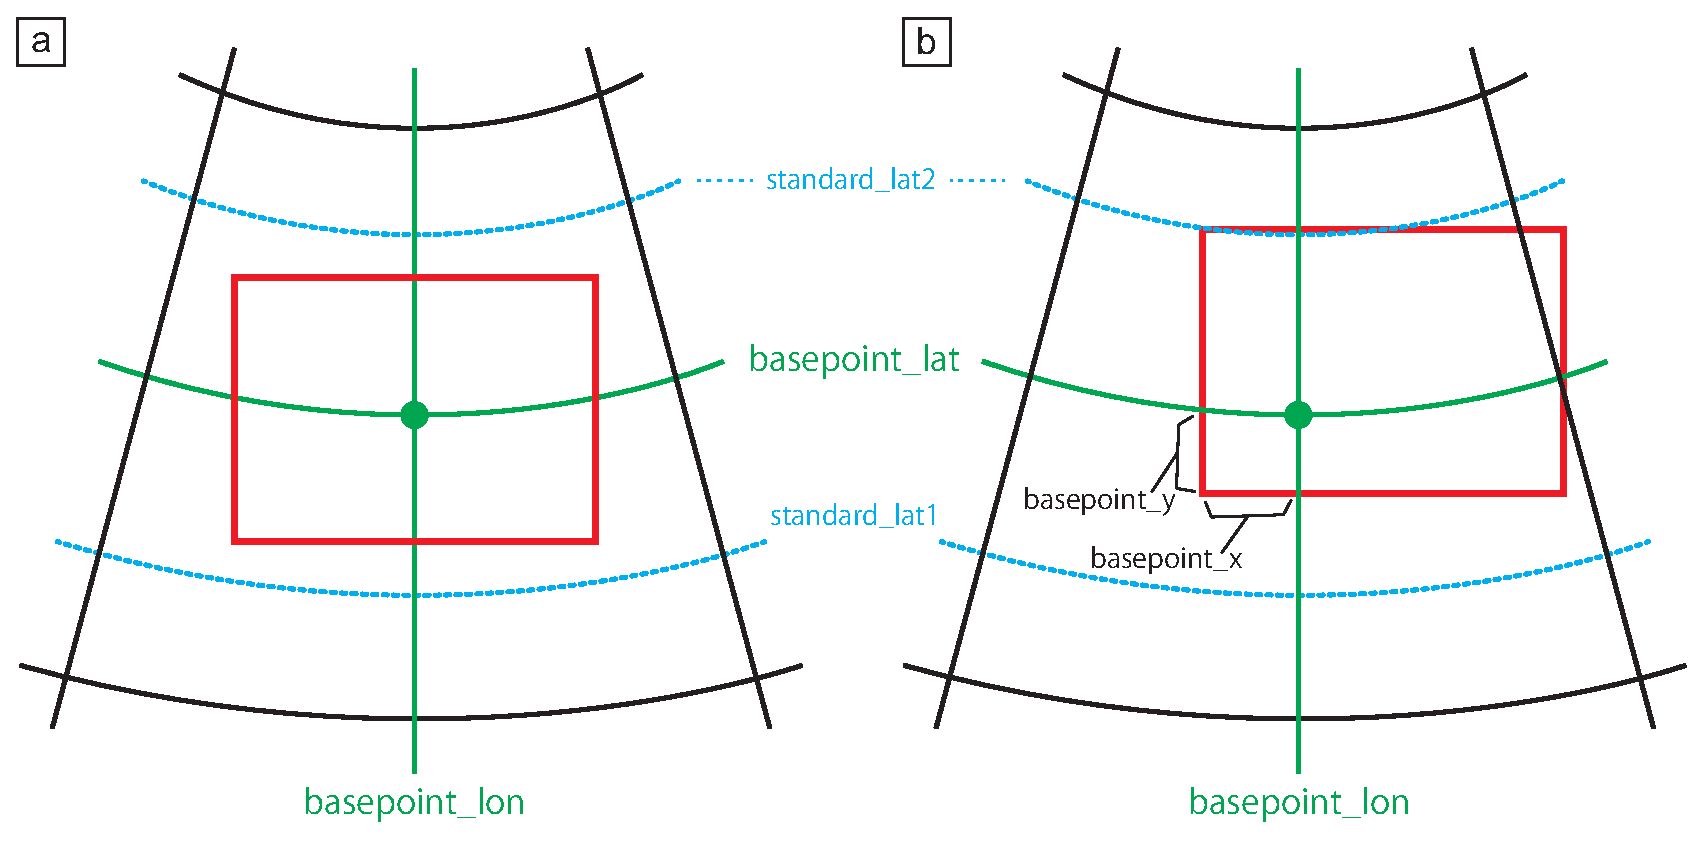
\includegraphics[width=0.8\hsize]{./figure/LC_latlon_xy.eps}\\
  \caption{投影中心と計算領域の関係:(a)はデフォルト設定の場合、(b)は計算領域の位置を投影中心からずらした場合。
  赤線の矩形が計算領域を表す。}
  \label{fig:map_lc}
\end{center}
\end{figure}


\section{側面境界条件} \label{sec:adv_lateralbnd}
%------------------------------------------------------
SCALEでは、側面境界条件として「周期境界条件」と「外部入力データ指定」の2種類から選択できる。デフォルトの設定は東西方向、
南北方向ともに周期境界条件となっている。主に理想実験では周期境界条件を使用し、現実大気実験では外部入力データ指定
を使用することを想定している。設定方法によっては、他の側面境界条件も設定可能であるが、現在のところ想定外の
使用方法であるためサポートできない。

側面境界条件の設定は、configファイルの\verb|PARAM_PRC|の項目を編集することで設定できる。
\textcolor{red}{\bf この設定は、pp\_***.conf、init\_***.conf、run\_***.confのconfigファイルの間で
必ず一致させなければならない。} 周期境界条件を設定したい場合は、デフォルト設定なので特にconfigファイルに記述する
必要はない。理想実験チュートリアルのconfigファイルの\verb|PARAM_PRC|の項目を見れば特に境界条件に関する記述が
ないことがわかるだろう。一方、外部入力データ指定を設定したい場合は、下記のように``\verb|PRERIODIC|''のスイッチを
``false''に指定する。\\

\noindent {\small {\gt
\ovalbox{
\begin{tabularx}{140mm}{l}
\verb|&PARAM_PRC| \\
\verb|      〜 中略 〜|\\
\verb| PRC_PERIODIC_X  = .false.,| \\
\verb| PRC_PERIODIC_Y  = .false.,| \\
\verb|/| \\
\end{tabularx}
}}}\\

\noindent 外部入力データ指定の場合は、\ref{sec:adv_gridspace}節で説明した必ず側面境界のバッファー領域を
設定しなければならない。バッファー領域でどの変数に強制をかけるか(ダンピングするか)、またその場合の時定数などの
設定はconfigファイルの\verb|PARAM_ATMOS_BOUNDARY|の項目で指定できる。現実大気実験のチュートリアルの
configファイル(\verb|run.conf|)を元にして一部の項目を説明する。\\

\noindent {\small {\gt
\ovalbox{
\begin{tabularx}{140mm}{l}
\verb|&PARAM_ATMOS_BOUNDARY|\\
\verb| ATMOS_BOUNDARY_TYPE        = "REAL",|\\
\verb| ATMOS_BOUNDARY_IN_BASENAME = "../init/boundary_d01",|\\
\verb| ATMOS_BOUNDARY_USE_VELZ    = .true.,|\\
\verb| ATMOS_BOUNDARY_USE_QHYD    = .false.,|\\
\verb| ATMOS_BOUNDARY_VALUE_VELZ  = 0.0D0,|\\
\verb| ATMOS_BOUNDARY_UPDATE_DT   = 21600.0D0,|\\
\verb|/|\\
\end{tabularx}
}}}\\

上2つの項目は、``REAL''が外部入力データを使用することを意味し、次の行の指定がその外部入力データのファイル名を指定している。
上から3つ目の設定項目である``\verb|ATMOS_BOUNDARY_USE_VELZ = .true.|''は、鉛直速度に対して「強制をかける」ことを
意味している。一方、``\verb|ATMOS_BOUNDARY_USE_QHYD = .false.|''として、凝結物の混合比に対しては逆に「強制をかけない」
設定になっている。その次の項目の``\verb| ATMOS_BOUNDARY_VALUE_VELZ|''は、鉛直速度に対して
強制をかける際、ここで指定した値、``0.0 m/s''へ近づくように強制をかけるという指定を意味する。
最後の行の``\verb|ATMOS_BOUNDARY_UPDATE_DT|''は、外部入力データの更新間隔が21600秒であることを
意味している。たとえば、6時間間隔でデータが与えられている再解析データを外部入力データとして使用する場合にこの設定になる。

他にも、水平速度東西成分(\verb|VELX|)、水平速度南北成分(\verb|VELY|)や温位(\verb|POTT|)などに対して同様の設定項目が
存在する。また、ダンピングの時定数を設定する\verb|ATMOS_BOUNDARY_TAUX|や\verb|ATMOS_BOUNDARY_TAUY|といった設定項目がある。
更なる詳細については、付録\ref{app:namelist}を参照のこと。


%と加える(どちらの変数もデフォルトはtrueで周期境界が用いられる).スポンジ層ではレイリーダンピングがかけられる.
%スポンジ層でかけるレイリーダンピングの設定はrun.confのPARAM\_ATMOS\_BOUNDARYで設定する.
%設定方法の一例とそれぞれのNamelistの意味を下に示す.
%\begin{verbatim}
% ATMOS_BOUNDARY_TYPE         = "INIT",  (初期値に近づくように緩和する)
% ATMOS_BOUNDARY_USE_VELZ     = .true., (速度の鉛直成分にダンピングを適用する)
% ATMOS_BOUNDARY_USE_VELX     = .true., (速度のx成分にダンピングを適用する)
% ATMOS_BOUNDARY_USE_VELY     = .true., (速度のy成分にダンピングを適用する)
% ATMOS_BOUNDARY_USE_POTT     = .true., (温位にダンピングを適用する)
% ATMOS_BOUNDARY_USE_QV       = .true., (温位にダンピングを適用する)
% ATMOS_BOUNDARY_TAUX         =  300.D0, (x方向のダンピングの時定数:300[sec])
% ATMOS_BOUNDARY_TAUY         =  300.D0, (y方向のダンピングの時定数:300[sec])
% ATMOS_BOUNDARY_TAUZ         =  10.D0,  (z方向のダンピングの時定数:300[sec])
%\end{verbatim}
%各Namelistの詳細はAppendixを参照されたい.


